\documentclass{article} % For LaTeX2e
\usepackage{nips12submit_e,times}
\usepackage{natbib}
\usepackage[pdftex]{graphicx}
%\documentstyle[nips12submit_09,times,art10]{article} % For LaTeX 2.09


\title{Binary Separation on Heterogeneous Image}

\author{
Fisher Yu \\
\texttt{fy@princeton.edu}
\And
Nanxi Kang \\
\texttt{nkang@princeton.edu} 
\And
Siyu Liu\\
\texttt{siyuliu@princeton.edu}
}

\newcommand{\fix}{\marginpar{FIX}}
\newcommand{\new}{\marginpar{NEW}}

\nipsfinalcopy % Uncomment for camera-ready version

\begin{document}


\maketitle

\section{Introduction}
refer~\citet{Besag74}
\section{Data}
We got our data from Google street view team and processed it to use
the images in our project. The data was collected by a car equiped
with 8 cameras and 3 laser scanners. Each of the laser scanner can scan 180 degree 2D
plane at each time. Two of the laser scanners scanned vertically and
the third one scanned horizontally. As the car moved, the car
positions were recored by global positioning system. Those positions
were adjusted by the scans of the horizontal laser scanner using SLAM
(Simultaneous localization and mapping) techniques to get the best
precision. The 3D position of each laser scan point can be
estimated based on the relative position between the car and laser
scanners and therefore a 3D point cloud can be built from the scans of
the vertical laser scanners. At the same time, the eight
cameras were taking pictures as the car moved. Although the cameras
were well calibrated, the images were taken by rolling shutters and
there are errors in terms of image projection model if we assume each
image were taken in a pinhole model.

Given the 3D point cloud and images, we project the points into the
images with the estimated point positions, camera poses and projection
matrices. Then we can get images like Figure~\ref{fig-data_image}.

\begin{figure}[h]
\begin{center}
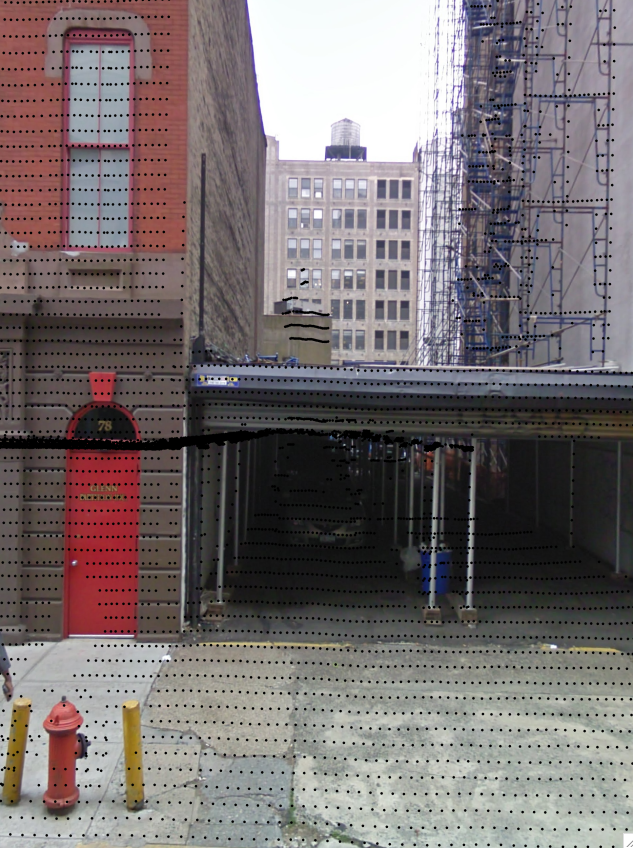
\includegraphics[height=0.5\linewidth]{./fig/image_sample.png}
\end{center}
\caption{An image with 3D points projected into it.}
\label{fig-data_image}
\end{figure}

In Figure~\ref{fig-data_image}, the black dots are the projections of
the 3D points in this image. As you can see, due to all kinds of
errors mentioned above, the 3D projections and the images are not well
aligned and we can't segment the images directly based on the depth of
the 3D scan points. In this project, we want to find the contour
between the background (the sky area) and foreground (all the objects
appears in the image, including roads and buildings). The models and
computing issue will be discussed in the methods section.

\section{Methods}

\section{Evaluation}
As explained before, the goal for this project is to separate the forground from background in street view images. However, provided ground truth is not available in our dataset, directly measuring the error seems not feasible (though we can measure the enery in the resulting MRF but it might not corresponding to the optimal behaviors as pointed out in \ref{Szeliski2008Comparative}). Thus, we plan to do a series of comparative expriments with current interactive methods mentioned in \ref{Szeliski2008Comparative}. Although modern MRF-based segmentation algorithms performs reasonably well, human facilitations during the process might be less favored in large dataset such as the street view dataset. Therefore,  by taking advantage of the LiDAR inputs, we are hoping to use sparse depth information as guidence to develop an automatic alternative yet competitive approach for binary image segmentation task. If our algorithm works as our optimistic estimation, we would attempt to generalize it into segmentation for multiple objects upon which we could further use these segments for image matching and possibly build models for 3D meshes for different objects accordingly. On the other hand, if the proposed method could not meet our expectation, we would like to explore the possibilities of reorganizing our lidar data as proper inputs for the interactive methods as in \ref{Rother2004GrabCut} and \ref{Arbelaez2011Contour}.

\bibliography{proposal}
\bibliographystyle{abbrvnat}


\end{document}
